\chapter{Der Weg zu DevOps} % Feel free to rename

Bis hierhin haben wir alles wichtige über DevOps gelernt. Seine Vor- und Nachteile, was es lösen kann und auch was es nicht lösen kann. Aber vorallem ist klar, dass DevOps nicht kaufbar ist. Zumindest nicht wie man eine Software kauft, installiert und dann vergessen kann. Darum gestaltet sich die Einführung von \ac{DevOps} in eine bereits bestehende Unternehmenskultur als schwierig.

Ein Ansatz um dieses Problem an zu gehen wird im nächsten Unterkapitel beschrieben.


\section{Der Three-Way-Approach}

Der Three-Way-Approach versucht sich an der Etablierung von \ac{DevOps} über 3 Stufen. \cite{nine:2018}

\begin{enumerate}
\item Das Flow Prinzip
\item Das Feedback Prinzip
\item Das Prinzip des kontinuierlichen Lernens und Experimentierens
\end{enumerate}

\begin{figure}[h]
\centering
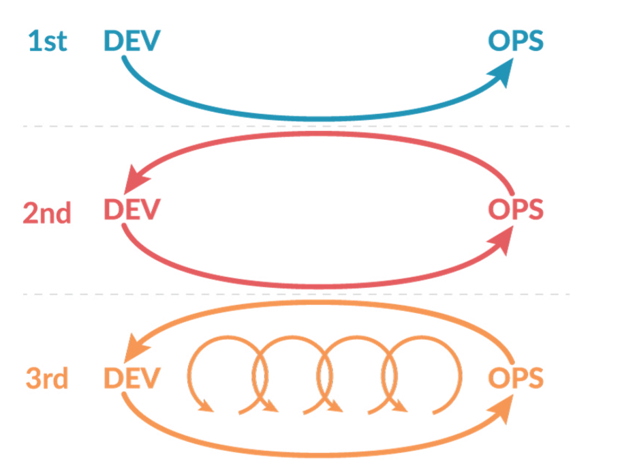
\includegraphics[width=0.6\textwidth]{Graphics/three_ways}
\caption{The Three Ways \cite{curra:2020}}
\end{figure}

Der erste Weg beschäftigt sich zu Beginn damit, den \textit{Flow} zwischen Prozessen zu verbessern. Gemeint ist damit die \glqq reibungslose, direkte Zusammenarbeit\grqq \cite{nine:2018}. Wichtig ist hierbei bereits Transparenz zu etablieren. Es muss eine Stelle geben, beispielsweise ein Sprint-Planning-Board oder ähnliches, über das alle Beteiligten auf einen Blick Einsicht erhalten über alle laufenden Prozesse, und vor allem auch wie dort der Fortschritt aussieht oder welche Probleme und Hindernisse es aktuell gibt.

\section{IDC DevOps Studie}
